\subsubsection*{Snow classification}
\label{sec:snow}

Snow is a somewhat unique visual phenomenon, and we claim that
detecting it in images is a unique recognition task. In some cases,
snow can be detected by coarse scene recognition: ski slopes or snowy
landscapes are distinctive scenes. But snow can appear in any kind of
outdoor scene, and is thus like an object. However, unlike most
objects that have some distinctive features, snow is simply a white,
near-textureless material.  (In fact, our informal observation is that
humans detect snow not by recognizing its appearance, but by noticing
that other expected features of a scene are occluded; in this sense,
detecting snow is less about the features that are seen and more about
the features that are \textit{not} seen. We leave this as an
observation to inspire future work.)
%
We tested a variety of off-the-shelf visual features for classifying
whether an image contains fallen snow. We used Support Vector
Machines for classification, choosing kernels based on the feature
type.  Intuitively, color is a very important feature for detecting
snow, and thus we focused on features that use color to at least some
degree. Our features include:


\xhdr{Color histograms} We begin with perhaps the simplest of color
features. We build joint histograms in CIELAB space, with 4 bins on
the lightness dimension and 14 bins along each of the two color
dimensions, for a total of 784 bins. We experimented with other
quantizations and found that this arrangement worked best.  We encode
the histogram as a 784 dimensional feature and use an SVM with a
chi-squared distance (as in~\cite{XiaoHEOT10}).

\xhdr{Tiny images} 
%Tiny images are another very simple way of
%representing an image that nevertheless capture coarse color and
%spatial layout information
We subsample images to 16 $\times$ 16 pixels, giving 256 pixels per
RGB color plane and yielding a 768 dimensional feature vector.
Drastically reducing the image dimensions yields a feature that is
less sensitive to exact alignment and more computationally
feasible~\cite{torralba2008tiny}.  
%We use an RBF kernel to compare the
%unnormalized distance.


\xhdr{Spatial Moments} Tiny images capture coarse color and spatial
scene layout information, but much information is discarded during
subsampling.  As an alternative approach, we convert the image to LUV
color space, divide it into 49 blocks using a 7 $\times$ 7 grid, and
then compute the mean and variance of each block in each color
channel.  Intuitively, this is a low-resolution image and a very
simple texture feature, respectively.  We also compute maximum,
minimum, and median value within each cell, so that the final
feature vector has 735 dimensions.
% The final feature vector
%thus has 7 $\times$ 7 $\times$ 3 $\times$ 5 = 735 dimensions.  We use
%an RBF kernel without normalization for this
%feature~\cite{boutell2005exploiting}.
%% dimension vector for a image. The distances are compared by RBF kernel
%% without normalization ~\cite{boutell2005exploiting}.

%%  We are most interested in the time and geo location of snow fall
%%  instead of generally finding snow in images. For example, snow
%%  mountain images are not expected to be classified as snow fall images
%%  first because it’s with snow all the time and second these images are
%%  always taken from a long distance away so the metadata of geo
%%  locations are hard to be trusted.  \pleasenote{ MK: I couldn't
%%    understand the relation between geo-time argument and spatial color
%%    in the image}.

%% In this case, spatial location appears to be important as well. And
%% this makes spatial color moments with CIE L*U*V* color space a very
%% important feature.  Both the CIE L*a*b* and L*U*V* spaces have good
%% approximate perceptual uniformity, but the L*U*V* has lower complexity
%% in its mapping. The Luv space has been shown to be effective for use
%% in multimedia applications ~\cite{furht1998multimedia}

%% After conversion to Luv space, the image is divided into 49 blocks
%% using a 7 x 7 grid. We compute the first and second moments (mean and
%% variance) of each Luv band, corresponding to a low‐resolution image
%% and to computationally‐inexpensive texture features,
%% respectively. Besides, we also add maximum, minimum and medium value
%% of each block each Luv band to Finally the feature is a 49 *3*5=735
%% dimension vector for a image. The distances are compared by RBF kernel
%% without normalization ~\cite{boutell2005exploiting}.

% \pleasenote{ MK: The following features are copied from placeavoider}.

%<<<<<<< .mine
\begin{figure*}[th!]
\begin{center}
\vspace{-16pt}
\begin{tabular}{cc}
 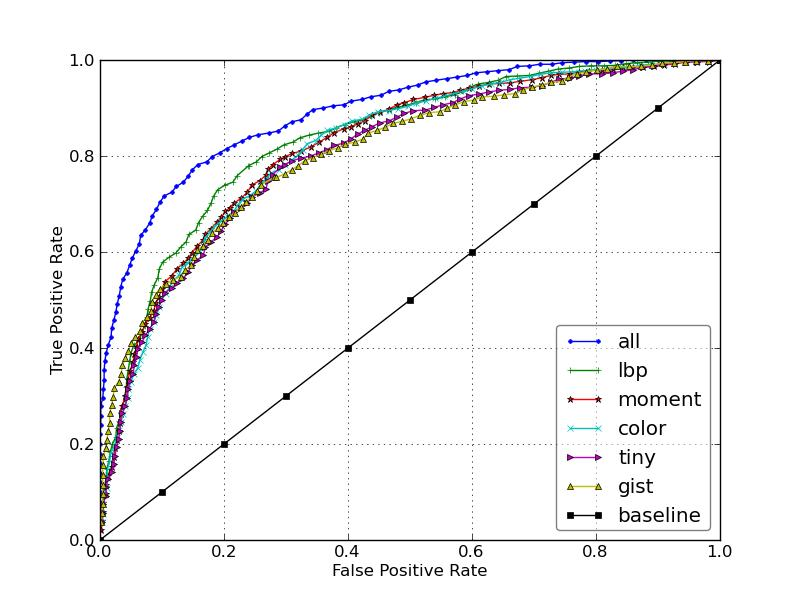
\includegraphics[width=0.4\textwidth]{figs/ROC-curves.jpg} &
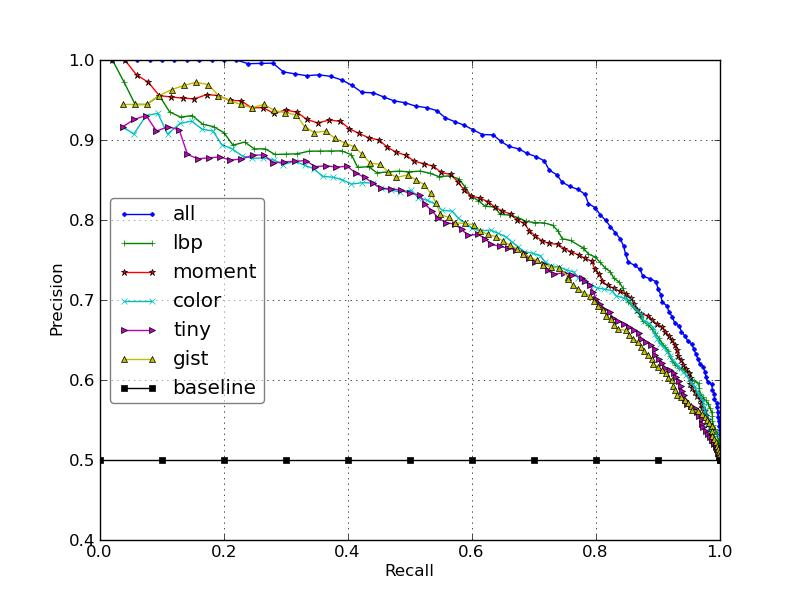
\includegraphics[width=0.4\textwidth]{figs/PR-curves.jpg} \\
\end{tabular}
\end{center}
\vspace{-8pt}
\caption{
Snow classification results for different features and combinations, in terms of {\textit{(left):}} ROC curves for the task of classifying snow vs. non-snow images; and 
{\textit{(right):}} Precision-Recall curves for the task of retrieving snow images.
}
\label{fig:PR_ROC_snow}
\end{figure*}
%=======
%\xhdr{{Color-informed Spatial Pyramid Local Binary Pattern (LBP):}} LBP converts
%each $9 \times 9$ pixel neighborhood of an image into an 8-bit binary
%number by thresholding the 8 outer pixels by the value of the center
%pixel.  We build a 256-bin histogram over these LBP values, both on
%the grayscale image and on each RGB color channel, to produce a
%1024-dimensional feature vector for each image~\cite{korayem2012solving}, then we build tow level spatial pyramid of lbp which generate 21504-dimensional feature vector for each image at the end.
%We use a an RBF kernel to compare these histograms. 
%\pleasenote{ MK: This different form place avoider because we build spatial pyramid of lbp }.
%>>>>>>> .r2679


\xhdr{{Color Local Binary Pattern (LBP) with pyramid
    pooling}} LBP represents each $9 \times 9$ pixel neighborhood 
as an 8-bit binary number by thresholding the 8 outer pixels
by the value at the center.  We build 256-bin histograms over
these LBP values, both on the grayscale image and on each RGB color
channel~\cite{korayem2012solving}. We compute these histograms in each cell of a three-level spatial
pyramid, with 1 bin at the lowest level, 4 bins in a $2 \times 2$ grid
at the second level, and 16 bins in a $4 \times 4$ grid at the third level.
This yields a $(1+4+16) \times 4 \times 256$ = 21504 dimensional feature
vector for each image.

\xhdr{GIST} We also apply GIST features, which capture coarse texture
and scene layout by applying a Gabor filter bank followed by
down-sampling~\cite{oliva2001modeling}, Our variant produces a
1536-dimensional feature vector and operates on color planes. Scaling
images to have square aspect ratios before computing GIST improved
classification results significantly; \cite{douze2009evaluation}
observed the same effect on a different problem.


We experimented with a number of other features, and found
that they did not work well; local features like SIFT and HOG in
particular perform poorly, again because snow does not have
distinctive visual appearance. 

\subsubsection*{Results}




\begin{table}[b]
\begin{center}
{\footnotesize{
\begin{tabular}{|l|c|c|}
\hline 
Feature & Kernel  & Accuracy\tabularnewline
\hline 
\hline 
Random Baseline  & --- & 50.0\%\tabularnewline
\hline 
\hline
Gist & RBF & 73.7\%\tabularnewline
\hline 
Color  & $\chi^2$ & 74.1\%\tabularnewline
\hline
Tiny & RBF & 74.3\%\tabularnewline
\hline 
Spatial Color Moments & RBF & 76.2\%\tabularnewline
\hline 
Spatial pyramid LBP & RBF &\textbf{77.0\%}\tabularnewline
\hline 
\hline
All features  & linear & \textbf{80.5\%}\tabularnewline
\hline 
\end{tabular}
}}
\caption{Performance of different features  for snow detection, all using SVMs for classification. }
\label{tab:snow}
\end{center}
\end{table}


We tested these approaches to detecting snow on our dataset of
10,000 hand-labeled images. We split this set into a training set of
8,000 images and a test set of 2,000 images, sampled to have an
 equal proportion of snow and non-snow images (so
that the accuracy of a random baseline is 50\%).
Table~\ref{tab:snow} presents the results. We observe that all of the
features perform significantly better than a random baseline. 
Gist, Color Histograms and Tiny Image all give very similar accuracies, within a half
percentage point of 74\%. Spatial Moments and
LBP  features perform
slightly better at 76.2\% and 77.0\%. We also tested a combination of all 
features by learning a second-level linear SVM on the output of the
five SVMs; this combination performed significantly better than any single feature,
at 80.5\%.


Figure~\ref{fig:PR_ROC_snow} shows classification performance in
terms of an ROC curve, as well as a
precision-recall curve in which the task is to retrieval photos
containing snow. The precision-recall curve shows that at about 20\%
recall, precision is very near to 100\%, while even at 50\% recall,
precision is close to 90\%.  This is a nice feature because in many
applications, it may not be necessarily to correct classify all
images, but instead to find some images that most likely contain a
subject of interest.
%
To give a sense for the difficulty and failure modes of our dataset,
we show a random sample of correct and incorrect classification results
in Figure~\ref{fig:fp}.

\xhdr{Reconstructing satellite snow maps} Finally, we tested whether
this automated photo classification run on large-scale collections of
geo-tagged, time-stamped social images could be used to approximate
snow maps generated by satellites.  An advantage of considering the
snow recognition task is that ground truth, in the form of daily snow
cover maps, is publicly available from NASA and
others~\cite{ecology2012www}. This is thus a somewhat artificial task
because very good datasets already exist for snow cover, but we use
this problem here as a test case of the more general idea of using
Flickr to observe nature. (Nevertheless, 
satellites are also limited because they require the ground to be
visible, and thus are not effective when there is cloud cover.)

To test this idea, we downloaded public, geo-tagged, time-stamped
Flickr photos taken in North America on three days: March 3, April 6,
and December 21 2009 (4422, 5606, and 9906 photos respectively).  We
ran our combined classifiers on these images. We discretized the image
geo-tags into 1 degree by 1 degree bins, and interpreted each snowy
image as evidence of snow in that bin and each non-snowy image as
evidence against snow in that bin. We combined this evidence together
using the simple Bayesian approach proposed by~\cite{ecology2012www}.
Figure~\ref{fig:satellite} shows the resulting map produced by our automated
Flickr analysis, and compares it to the corresponding snow cover map
produced by NASA's MODIS instrument~\cite{modissnow}. We note that
the Flickr map is much sparser than the satellite map, especially in 
sparsely populated areas like northern Canada and the western U.S. On
the other hand, the Flickr maps give some observations even when the
satellite maps are missing data due to clouds.

\begin{figure}[t]
\begin{center}
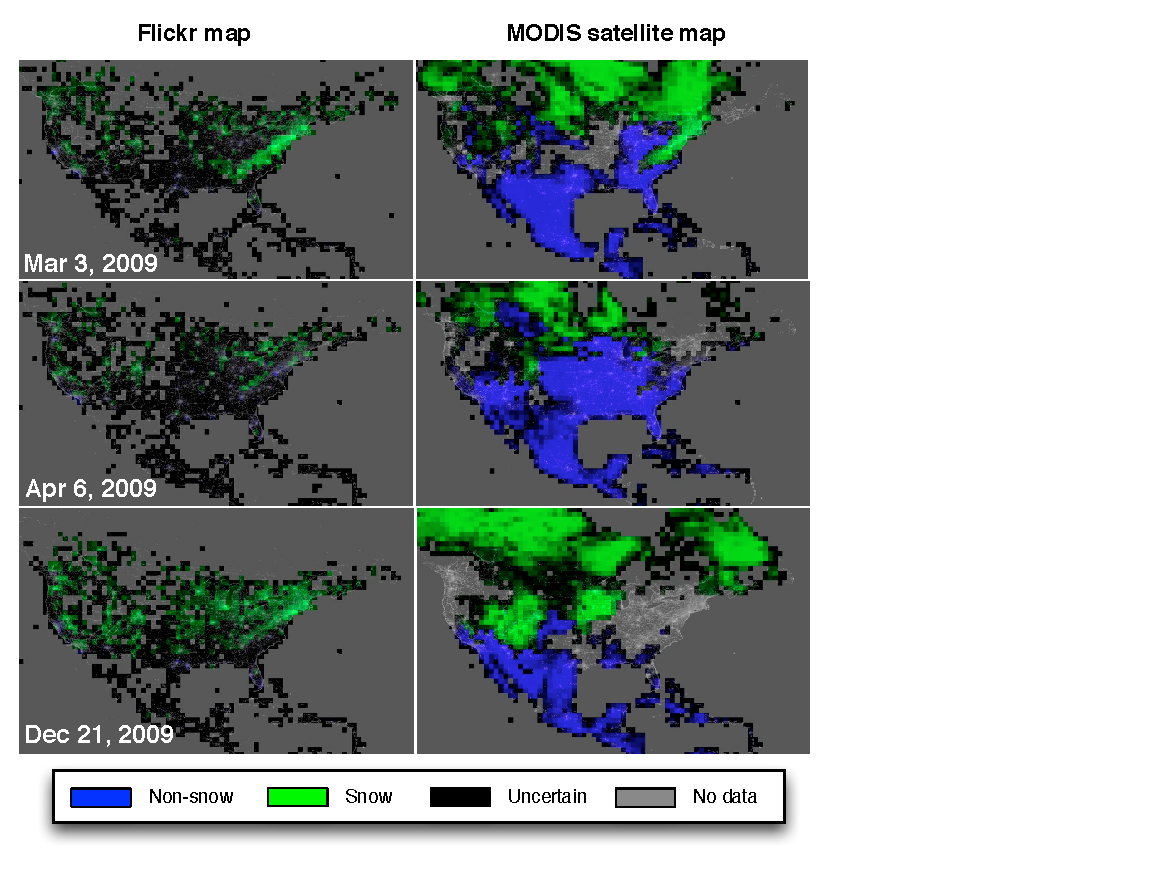
\includegraphics[width=0.46\textwidth,trim=0.2cm 0.7cm 6cm 0cm,clip]{figs/satellite-map.pdf}
\end{center}
\vspace{-12pt}
\caption{Automatically-generated snow cover maps generated by our
Flickr analysis (left), compared with actual satellite maps (right),
for three days.}
\label{fig:satellite}
\vspace{-8pt}
\end{figure}

%%%%%%%% mk: 10 images for snow images True positive . Snow images classified as snow
 
\begin{figure*}[th]
{\small{
\begin{center}
\begin{tabular}{@{}c@{\,\,\,}c@{\,\,\,}c@{\,\,\,}c@{\,\,\,}c@{\,\,\,}}
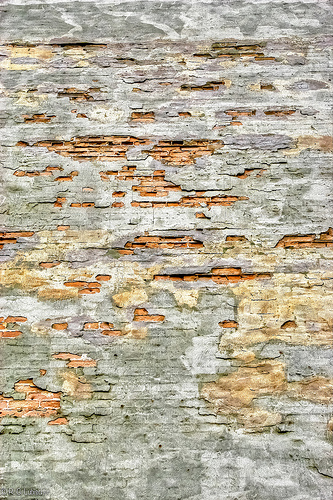
\includegraphics[height=1.05in]{figs/tn1.jpg} &
%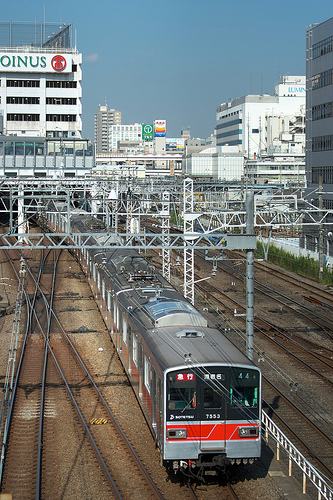
\includegraphics[height=1in]{figs/tn2.jpg} &
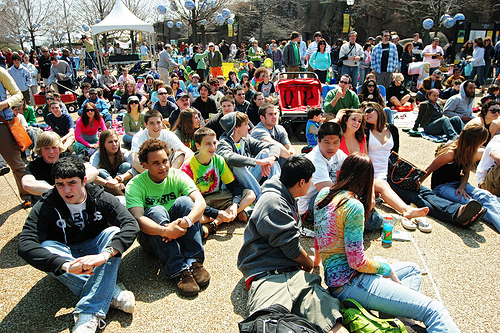
\includegraphics[width=0.19\textwidth]{figs/tn3.jpg} &
%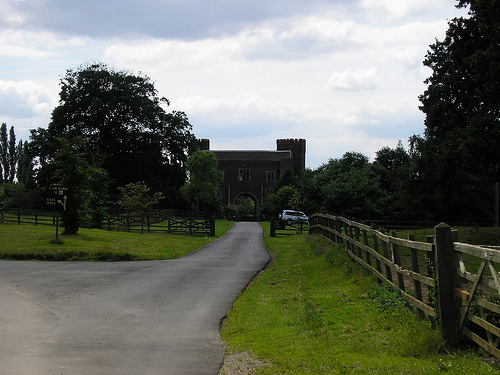
\includegraphics[width=0.19\textwidth]{figs/tn4.jpg} &
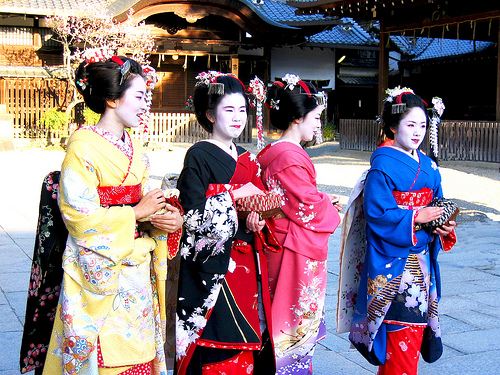
\includegraphics[width=0.19\textwidth]{figs/tn5.jpg} &
%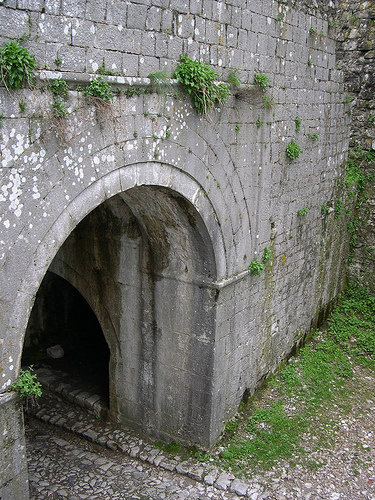
\includegraphics[height=1in]{figs/tn6.jpg} &
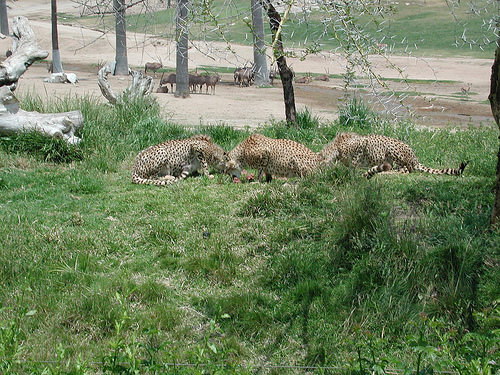
\includegraphics[width=0.19\textwidth]{figs/tn7.jpg} &
%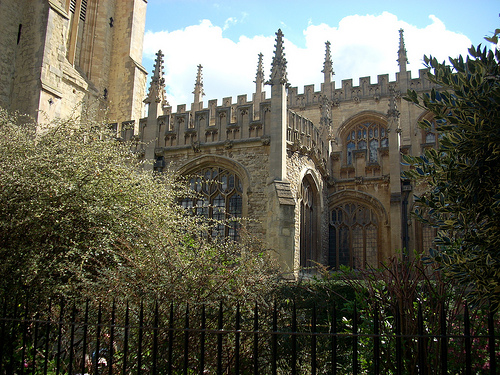
\includegraphics[width=0.19\textwidth]{figs/tn8.jpg} &
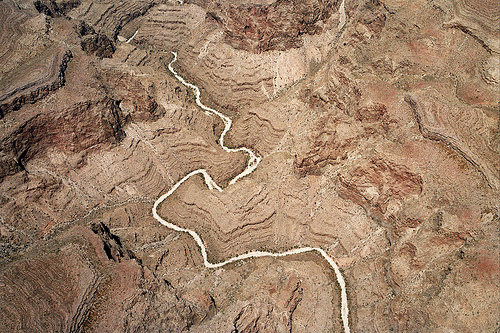
\includegraphics[width=0.19\textwidth]{figs/tn9.jpg} \\
%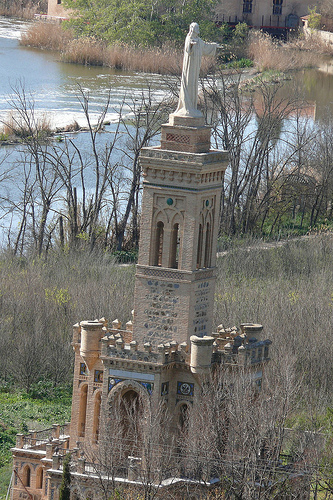
\includegraphics[height=1in]{figs/tn10.jpg} \\
\multicolumn{5}{c}{(a) Random true negatives (non-snow images classified as non-snow)} \\
\\[-6pt]
 \hline
\\[-6pt]
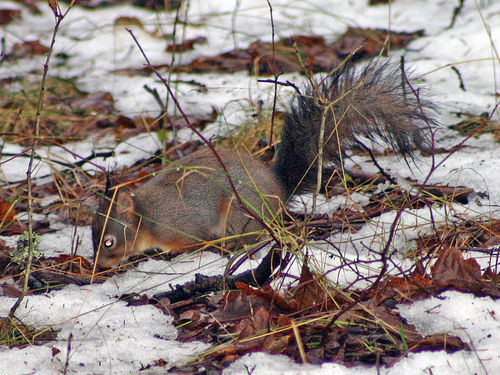
\includegraphics[width=0.19\textwidth]{figs/tp1.jpg} &
%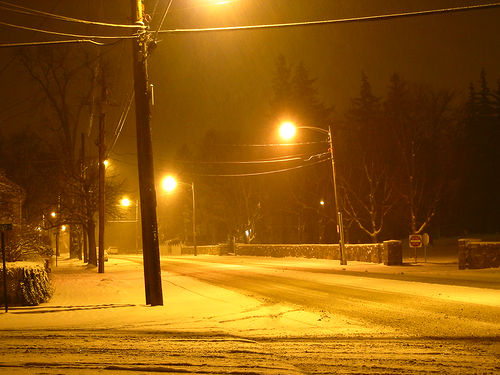
\includegraphics[width=0.19\textwidth]{figs/tp2.jpg} &
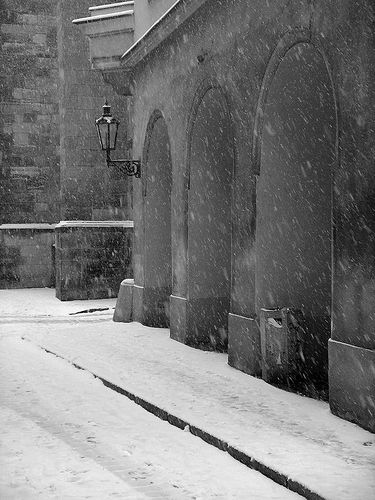
\includegraphics[height=1.05in]{figs/tp3.jpg} &
%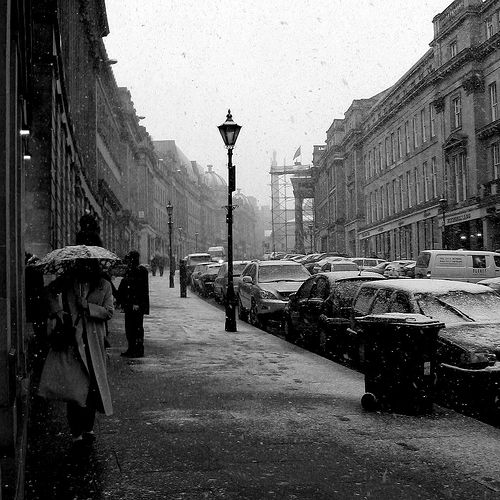
\includegraphics[width=0.19\textwidth]{figs/tp4.jpg} &
%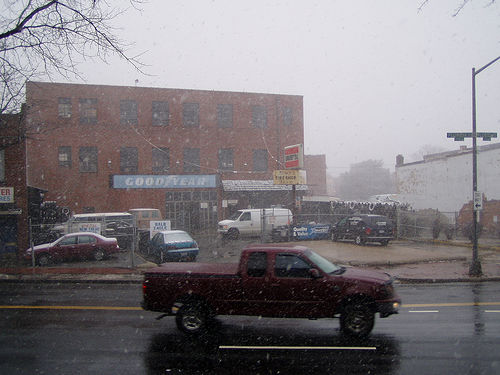
\includegraphics[width=0.19\textwidth]{figs/tp5.jpg} &
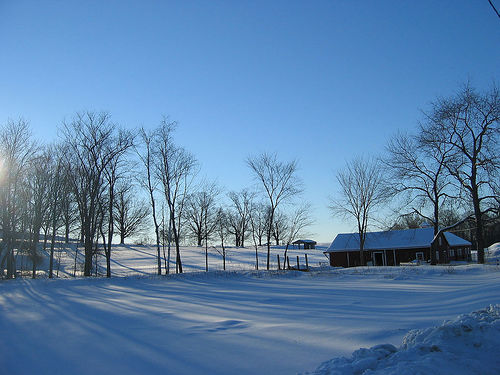
\includegraphics[width=0.19\textwidth]{figs/tp6.jpg} &
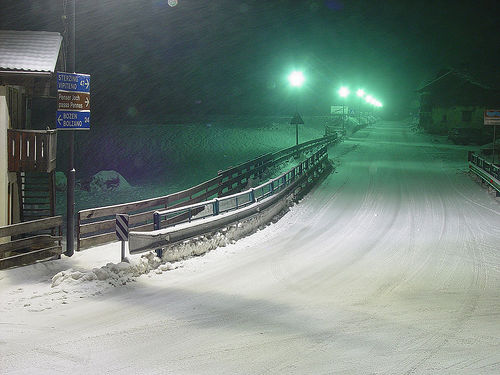
\includegraphics[width=0.19\textwidth]{figs/tp7.jpg} &
%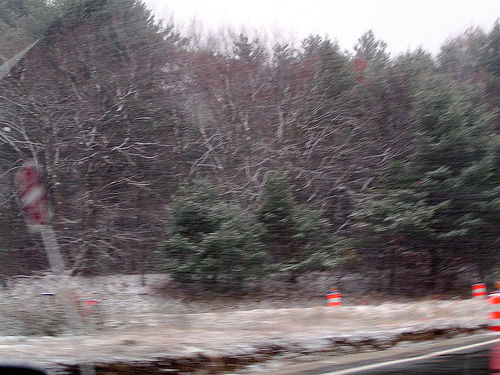
\includegraphics[width=0.19\textwidth]{figs/tp8.jpg} &
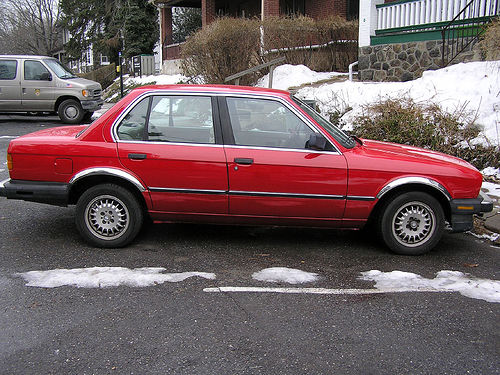
\includegraphics[width=0.19\textwidth]{figs/tp9.jpg} \\
%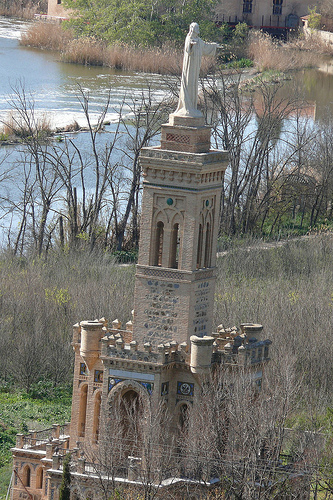
\includegraphics[width=0.19\textwidth]{figs/tn10.jpg} \\
\multicolumn{5}{c}{(b) Random true positives (snow images classified as snow)} \\ 
\\[-6pt]
\hline
\\[-6pt]
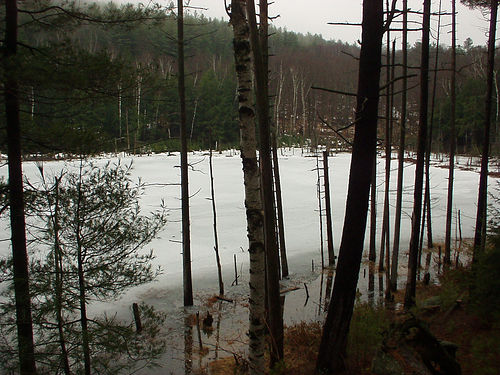
\includegraphics[width=0.19\textwidth]{figs/fp1.jpg} &
%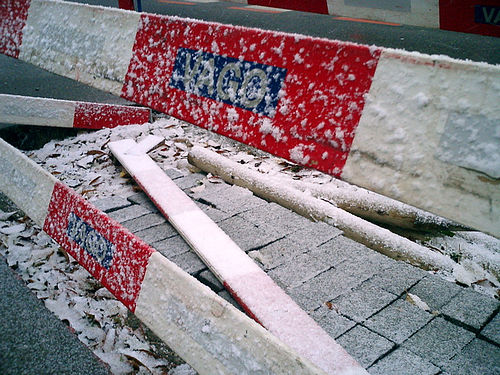
\includegraphics[width=0.19\textwidth]{figs/fp2.jpg} &
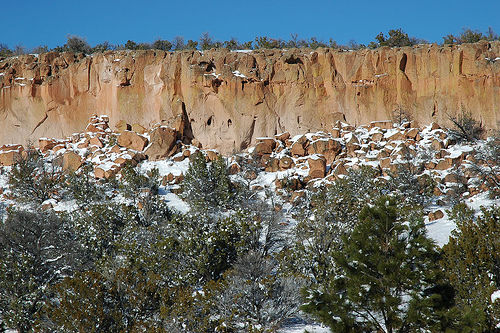
\includegraphics[width=0.19\textwidth]{figs/fp3.jpg} &
%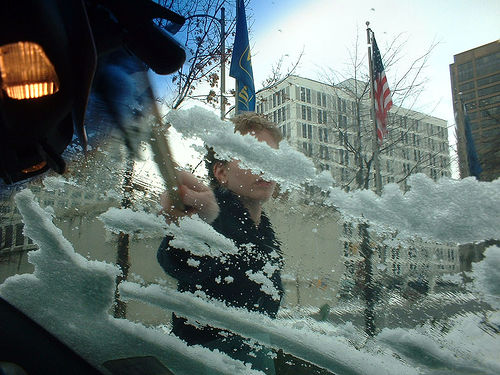
\includegraphics[width=0.19\textwidth]{figs/fp4.jpg} &
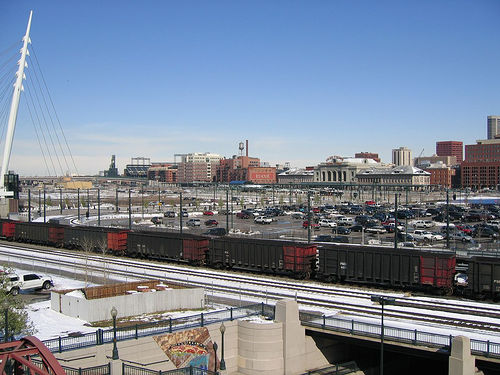
\includegraphics[width=0.19\textwidth]{figs/fp5.jpg} &
%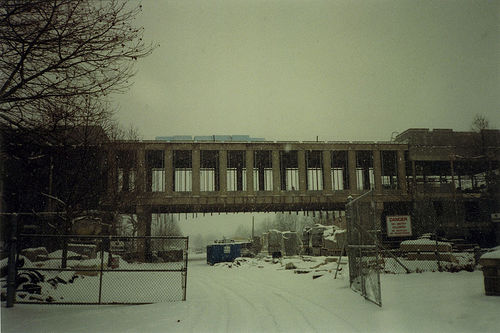
\includegraphics[width=0.19\textwidth]{figs/fp6.jpg} &
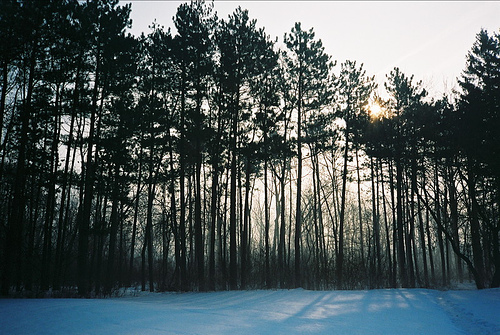
\includegraphics[width=0.19\textwidth]{figs/fp7.jpg} &
%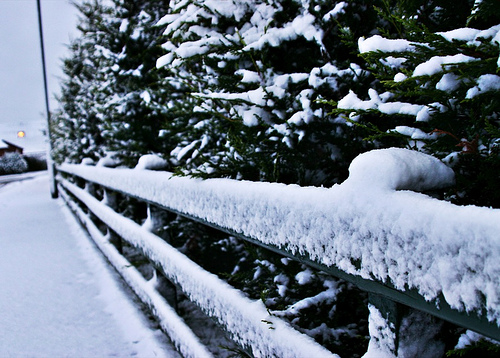
\includegraphics[width=0.19\textwidth]{figs/fp8.jpg} &
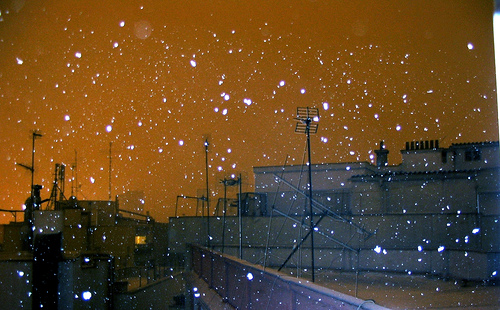
\includegraphics[width=0.19\textwidth]{figs/fp9.jpg} \\
%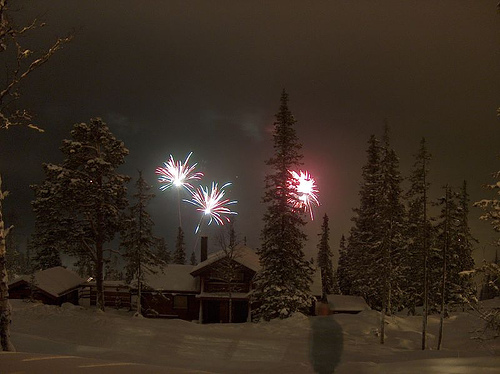
\includegraphics[width=0.19\textwidth]{figs/fp10.jpg} \\
\multicolumn{5}{c}{(c) Random false negatives (snow images classified as non-snow)} \\ 
\\[-6pt]
\hline
\\[-6pt]
%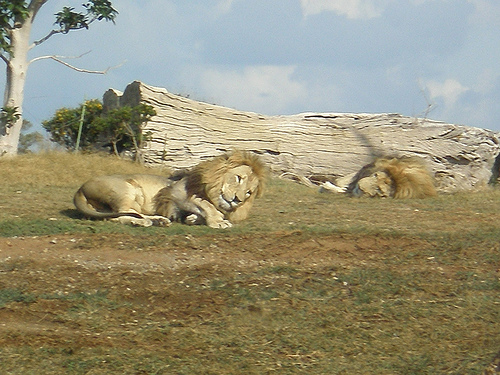
\includegraphics[width=0.19\textwidth]{figs/fn1.jpg} &
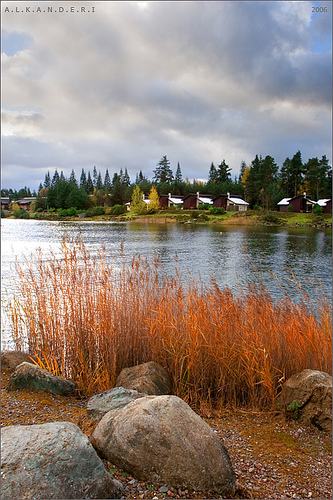
\includegraphics[height=1.05in]{figs/fn2.jpg} &
%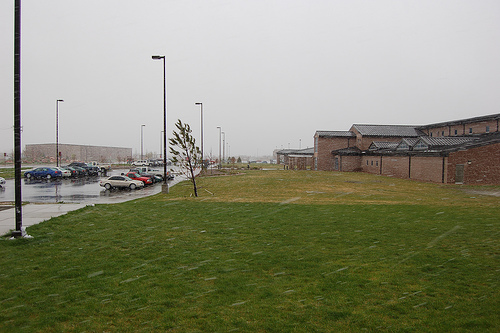
\includegraphics[width=0.19\textwidth]{figs/fn3.jpg} &
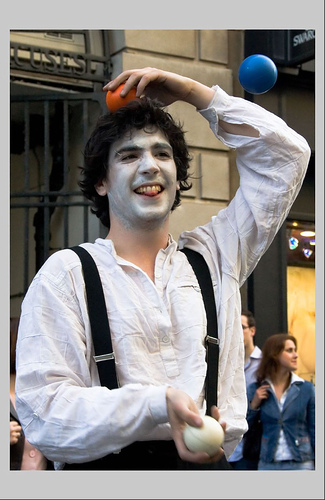
\includegraphics[height=1.05in]{figs/fn4.jpg} &
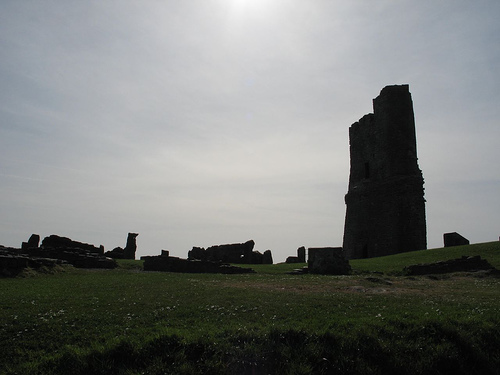
\includegraphics[width=0.19\textwidth]{figs/fn5.jpg} &
%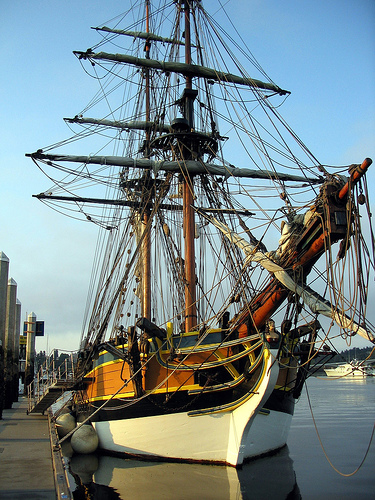
\includegraphics[width=0.19\textwidth]{figs/fn6.jpg} &
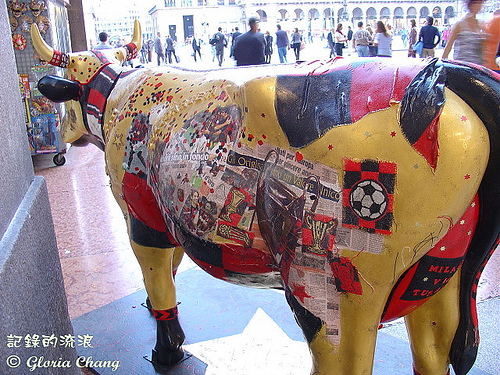
\includegraphics[width=0.19\textwidth]{figs/fn7.jpg} &
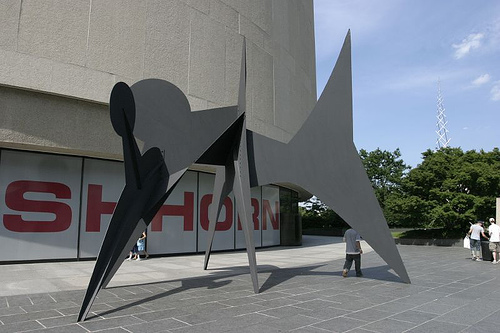
\includegraphics[width=0.19\textwidth]{figs/fn8.jpg} \\
%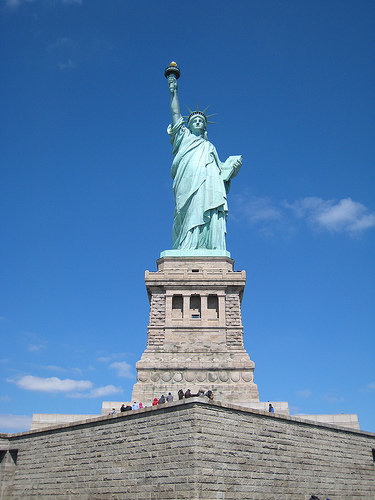
\includegraphics[height=1.1in]{figs/fn9.jpg} \\
%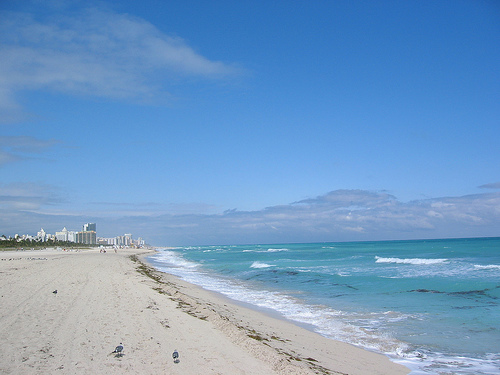
\includegraphics[width=0.19\textwidth]{figs/fn10.jpg} \\
\multicolumn{5}{c}{(d) Random false positives (non-snow images classified as snow)} \\
\end{tabular}
\end{center}
}}
\caption{Snow classification results on some random images from our dataset, including (from top) true negatives, true positives, false negatives, and false positives.
These results were obtained using the combined classifier that uses all of the image features.}
\label{fig:fp}
\end{figure*}



%% %%%%%%%% mk: 10 images for snow images True positive . Snow images classified as snow
 
%% \begin{figure*}[th]
%% \begin{center}
%% \begin{tabular}{ccccc}
%% 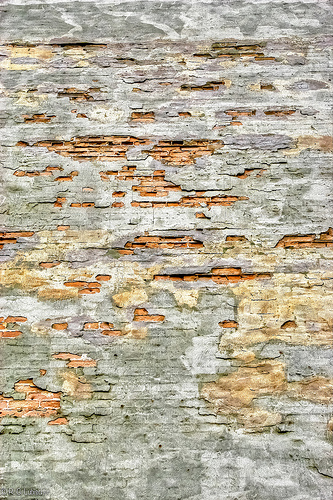
\includegraphics[height=1in]{figs/tn1.jpg} &
%% 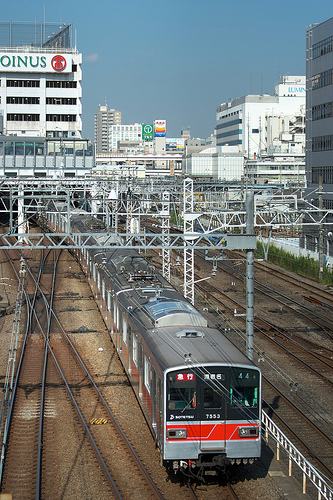
\includegraphics[height=1in]{figs/tn2.jpg} &
%% 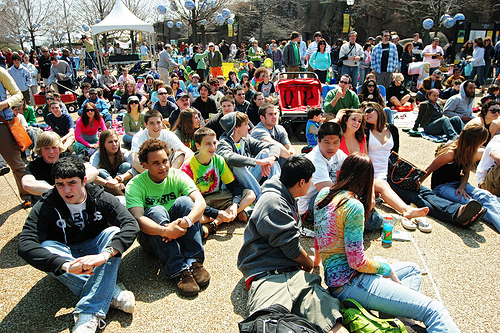
\includegraphics[width=0.19\textwidth]{figs/tn3.jpg} &
%% 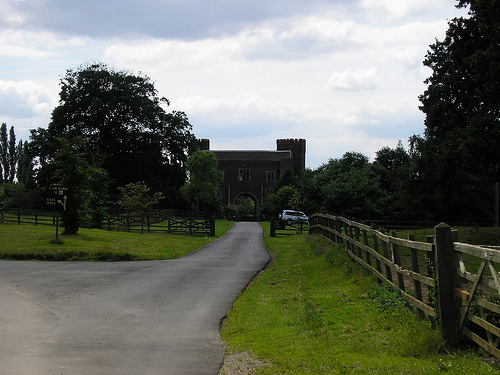
\includegraphics[width=0.19\textwidth]{figs/tn4.jpg} &
%% 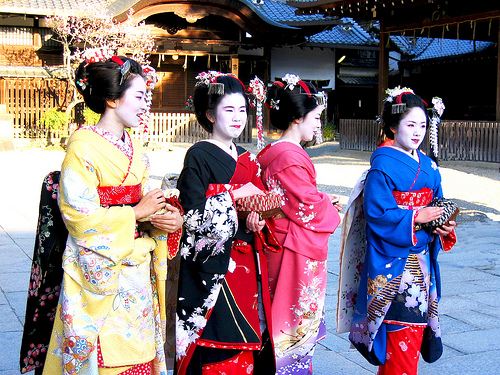
\includegraphics[width=0.19\textwidth]{figs/tn5.jpg} \\

%% 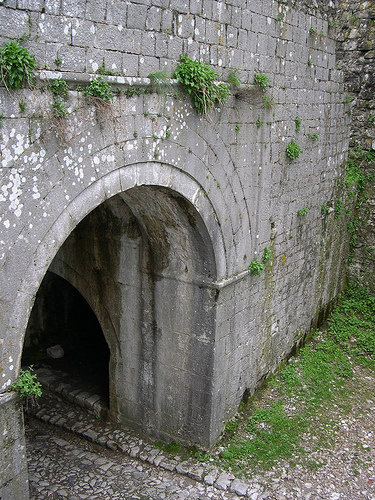
\includegraphics[height=1in]{figs/tn6.jpg} &
%% 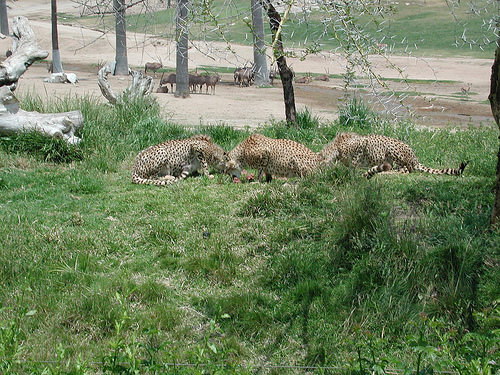
\includegraphics[width=0.19\textwidth]{figs/tn7.jpg} &
%% \includegraphics[width=0.19\textwidth]{figs/tn8.jpg} &
%% \includegraphics[width=0.19\textwidth]{figs/tn9.jpg} &
%% \includegraphics[height=1in]{figs/tn10.jpg} \\

%% \end{tabular}
%% \end{center}
%% \caption{ 10 random images for  true negative , non snow images classified as non-snow  }
%% \label{fig:snow_TN}
%% \end{figure*}



%% %%%%%%%% mk: 10 images for snow images True positive . Snow images classified as snow
 
%% \begin{figure*}[th]
%% \begin{center}
%% \begin{tabular}{ccccc}
%% \includegraphics[width=0.19\textwidth]{figs/tp1.jpg} &
%% \includegraphics[width=0.19\textwidth]{figs/tp2.jpg} &
%% \includegraphics[width=0.19\textwidth]{figs/tp3.jpg} &
%% \includegraphics[width=0.19\textwidth]{figs/tp4.jpg} &
%% \includegraphics[width=0.19\textwidth]{figs/tp5.jpg} \\

%% \includegraphics[width=0.19\textwidth]{figs/tp6.jpg} &
%% \includegraphics[width=0.19\textwidth]{figs/tp7.jpg} &
%% \includegraphics[width=0.19\textwidth]{figs/tp8.jpg} &
%% \includegraphics[width=0.19\textwidth]{figs/tp9.jpg} &
%% \includegraphics[width=0.19\textwidth]{figs/tn10.jpg} \\

%% \end{tabular}
%% \end{center}
%% \caption{ 10 random images for  true positive ,  snow images classified as snow  }
%% \label{fig:snow_TP}
%% \end{figure*}



%% %%%%%%%% mk: 10 images for snow images flase positive . Snow images classified as non-snow
 
%% \begin{figure*}[th]
%% \begin{center}
%% \begin{tabular}{ccccc}
%% \includegraphics[width=0.19\textwidth]{figs/fp1.jpg} &
%% \includegraphics[width=0.19\textwidth]{figs/fp2.jpg} &
%% \includegraphics[width=0.19\textwidth]{figs/fp3.jpg} &
%% \includegraphics[width=0.19\textwidth]{figs/fp4.jpg} &
%% \includegraphics[width=0.19\textwidth]{figs/fp5.jpg} \\

%% \includegraphics[width=0.19\textwidth]{figs/fp6.jpg} &
%% \includegraphics[width=0.19\textwidth]{figs/fp7.jpg} &
%% \includegraphics[width=0.19\textwidth]{figs/fp8.jpg} &
%% \includegraphics[width=0.19\textwidth]{figs/fp9.jpg} &
%% \includegraphics[width=0.19\textwidth]{figs/fp10.jpg} \\

%% \end{tabular}
%% \end{center}
%% \caption{ 10 random images for  false positive ,  snow images classified as non-snow  }
%% \label{fig:fp}
%% \end{figure*}



%% %%%%%%%% mk: 10 images for snow images flase negative .  NON Snow images classified as snow
 
%% \begin{figure*}[th]
%% \begin{center}
%% \begin{tabular}{ccccc}
%% \includegraphics[width=0.19\textwidth]{figs/fn1.jpg} &
%% \includegraphics[width=0.19\textwidth]{figs/fn2.jpg} &
%% \includegraphics[width=0.19\textwidth]{figs/fn3.jpg} &
%% \includegraphics[width=0.19\textwidth]{figs/fn4.jpg} &
%% \includegraphics[width=0.19\textwidth]{figs/fn5.jpg} \\

%% \includegraphics[width=0.19\textwidth]{figs/fn6.jpg} &
%% \includegraphics[width=0.19\textwidth]{figs/fn7.jpg} &
%% \includegraphics[width=0.19\textwidth]{figs/fn8.jpg} &
%% \includegraphics[width=0.19\textwidth]{figs/fn9.jpg} &
%% \includegraphics[width=0.19\textwidth]{figs/fn10.jpg} \\

%% \end{tabular}
%% \end{center}
%% \caption{ 10 random images for  false negative ,  non-snow images classified as snow  }
%% \label{fig:fp}
%% \end{figure*}
